\chapter{Background: GDPR and the Semantic Web}
\label{chapter:background}

This chapter presents the necessary background information for understanding the research presented in this thesis. In particular, it presents a short introduction to the General Data Protection Regulation (GDPR) in \autoref{sec:background:GDPR} and to the Semantic Web in \autoref{sec:background:semweb}. The information represents a summary of these topics and is accompanied with links in the footnotes for further information.

\section{General Data Protection Regulation (GDPR)}\label{sec:background:GDPR}
The General Data Protection Regulation (GDPR) \cite{Regulation_GDPR} is the current data protection law applicable within the European Union (EU) and the European Economic Area (EEA) and regulates use and processing of personal data. 
It supersedes its predecessor - the Data Protection Directive (DPD) \cite{directive_DPD} - and provides greater requirements and transparency for compliance, with potentially large and significant amount in fines if organisations are found to have violated its obligations.
A significant aspect of GDPR are its principles and rights which are intended to afford greater privacy and control to an individual regarding use of their personal data.

By virtue of being a regulation as opposed to a directive, GDPR is considered enforceable law with local and national data protection laws acting in conjunction rather than replacing it.
The GDPR has attracted global attention and scrutiny due to its requirements for compliance and potential fines, as well as for providing rights that enhance privacy.
It has influenced other privacy laws across the globe with the California Consumer Protection Act (CCPA) being a recent example \cite{marini_gdpr_2018}.

\subsection{Terminology}
The legal terminology utilised in GDPR is intended to clarify the roles, actions, and concepts referred in its obligations.
The definition of \textit{\textbf{personal data}} (Article 4-1) is based on linking, association, or relevance of any information with an individual - and represents a significant change from its predecessor as well from other laws which rely upon the concept of Personally Identifiable Information (PII). The individual the personal data relates to is termed as \textit{\textbf{Data Subject}} (Article 4-1) - a distinct term from other relevant laws that use \textit{individual} or \textit{PII Principal}.

GDPR regulates \textit{\textbf{processing}} of personal data (Article 4-1) - which is defined as any action over or utilising personal data as: ``collection, recording, organisation, structuring, storage, adaptation or alteration, retrieval, consultation, use, disclosure by transmission, dissemination or otherwise making available, alignment or combination, restriction, erasure or destruction;'' \cite{Regulation_GDPR}.

A \textit{\textbf{Controller}} is defined (Article 4-7) as the entity or organisation that determines \textit{\textbf{purpose}} and means of processing of personal data. As such, controller is the primary organisation regarding GDPR compliance and is subject to additional obligations given its role in determining processing of personal data. One or more controllers can act together to determine purpose and processing, in which case they are defined as \textit{\textbf{Joint-Controllers}} (Article 26).

A \textit{\textbf{Processor}} is defined (Article 4-8) as an entity which processes personal data on specified instructions of a controller (Article 28) and is not allowed to deviate from the instructions or utilise the personal data for other purposes. A processor is also referred to as \textit{(sub-)contractor} in some contexts. A processor may appoint other \textit{sub-processors} in order to carry out processing, where sub-processors are required to follow the same obligations as the processor.

A \textit{\textbf{Data Protection Officer (DPO)}} is defined (Article 37) as an individual appointed by a controller or processor to oversee compliance and processing of personal data, monitor internal processors, and collaborate with supervisory authorities as required.

A \textit{\textbf{Regulatory or Supervisory Authority or Data Protection Commission}} is a governmental organisation with responsibility to evaluate and enforce GDPR compliance. These bodies are established by national or federal governments and have jurisdiction over their appointed regions. The GDPR specifies responsibilities of such bodies and provides avenues for their co-operation across jurisdictions (Article 56, 60, 62).

GDPR provides several \textbf{\textit{rights}} to the data subject (Chapter 3) which are obligated to be provided by controller(s). Since rights are mandatory - their implementation, provision, and exercising must be monitored as part of compliance.

\textit{\textbf{Lawful Basis}} or \textit{\textbf{Legal Basis}} is the provision under which processing of personal data is permitted by GDPR, of which there are six primary ones (Article 6). \textit{Legitimate Interest} refers to legal basis where controller or third party needs personal data in order to provide or carry out its operations and services (Article 6-1f). Other legal basis include the carrying out a contract (Article 6-1b), compliance to legal obligation (Article 6-1c), public interest or as part of official authority (Article 6-1d), and other provisions and specifics introduced by national governments (Article 6-2).
\textit{\textbf{Consent of the Data Subject}} is the legal basis to be used where other legal basis are not applicable, and which requires consent of  data subject. Consent is subject to further obligations and requirements depending on the use-case which determine its validity.

\subsection{Transparency and Requirements}
Controllers are required to provide information to data subjects about processing activities regarding type of processing taking place and who is carrying it out.
This information is usually part of `privacy policy' and contains: (a) identity of controller(s); (b) purpose of processing; (c) legal basis; (d) transfer of data and categories of recipients; (e) data storage periods; and (f) the existence of rights.

In addition to above, a controller is required to monitor and maintain documentation detailing their processing of personal data categories along with particulars of data included within each category. Every personal data being processed must be associated with a source. GDPR specifies certain personal data categories as `special categories' based on their sensitivity and need for additional measures regarding security and accountability. Such special categories contain additional obligations for compliance which must be enforced if an organisation is using them. 

\subsection{Data Protection Impact Assessment}
A \textit{\textbf{Privacy Impact Assessment}} or \textit{\textbf{Data Protection Impact Assessment}} is an obligation of the controller to conduct and document an impact assessment of data processing before it is executed (Article 35). GDPR lays out conditions under which a DPIA is mandatory to be conducted - which includes processing that results in a high risk to rights and freedoms of data subjects, use of special categories of personal data, automated processing with significant effects, and use of evaluation or scoring.

A DPIA can be conducted for a specific processing activity, for a project, or for the entire organisation - and must be carried out ``prior to the processing'' (Articles 35-1, 35-10).
The aim of DPIA is to identify and mitigate data protection risks, plan for implementation of solutions to those risks, and assess viability of a project at an early stage.
Documentation of DPIA process allows demonstrating compliance with GDPR and minimising risks of legal difficulties in carrying out the processing.

Carrying out DPIA requires identification of information flows in terms of collection, storage, usage, sharing, and erasure of personal data within defined processing activities. A DPIA needs to be updated or carried out again if there are changes in processing activities.

\subsection{Sources of Additional Information}

\subsubsection{Data Protection Authorities}
A \textit{\textbf{Data Protection Authority (DPA)}} is the authority responsible for upholding EU laws and rights regarding privacy and data protection through enforcement and monitoring of compliance.
Its title and reference differs by language and jurisdiction - for example the \textit{Data Protection Commission (DPC)} in Ireland is also sometimes referred to as \textit{Data Protection Commissioner's Office}. 
A DPA is also referred to as \textit{Regulator} given their task of regulating processing of personal data.
In some nations (such as Germany) the data protection authorities are established in federal states or regions rather than a singular nation-wide office. The data protection authorities are also governed by national data protection laws in addition to the EU laws such as GDPR, and are responsible for their upholding as well.

The data protection authorities in each of their jurisdictions have published guidance and documents for assisting organisations and data subjects in understanding the GDPR and its compliance requirements. The authorities in Ireland\footnote{\url{https://www.dataprotection.ie/}}, United Kingdom\footnote{\url{https://ico.org.uk/}}, and France\footnote{\url{https://www.cnil.fr/en/home}} have provided this information in English.

\subsubsection{Article 29 Data Protection Working Party and European Data Protection Board (EDPB)}
The Article 29 Working Party (Art. 29 WP) was an advisory body to the European Parliament and its bodies, and consisted of representatives from data protection authorities of each EU member state, the European Data Protection Supervisor, and the European Commission. 
The body was established following the Data Protection Directive (DPD) and was replaced by European Data Protection Board (EDPB) under GDPR. 
The working party provided expert advice to member states, and published opinions on application of laws affecting right to protection of personal data - including the GDPR.
To this end, it published\footnote{\url{https://ec.europa.eu/justice/article-29/documentation/index_en.htm}} a number of documents clarifying or expressing opinions on interpretation of GDPR.

The EDPB is the European body replacing the Art. 29 WP with the purpose to ensure consistent application of GDPR and to assist in co-operation between various data protection authorities. 
EDPB is tasked with issuing guidelines, recommendations, and identifying best practices related to interpretation and application of GDPR.
It advises the European Commission on matters related to protection of personal data in EU and EEA by adopting consistency in cross-border cases, encouraging development of codes of conduct, establishing certification mechanisms for data protection, and promoting cooperation and effective exchange of information and good practices among national supervisory authorities. 
The EDPB has published\footnote{\url{https://edpb.europa.eu/edpb_en}} documents for providing information and assistance to individuals, controllers \& processors, and regulators.

% \subsubsection{Case Law, Legal Opinions, and Investigations}
% case law, opinions of legal authorities, fines and investigations by data protection authorities (website GDPR fine tracker)

\subsubsection{STAR \& STAR II}
STAR\footnote{\url{https://projectstareu.wordpress.com/}} (Support Training Activities on the data protection Reform) was an European project that provided materials to support training of DPAs and DPOs for GDPR.
Its resources are published in an open and publicly accessible form\footnote{\url{http://www.project-star.eu/training-materials}}. The project has produced a handbook for assisting stakeholders in understanding GDPR and preparing for its compliance. The project also provides an evaluation questionnaire and compliance checklist \cite{GDPR_compliance_checklist_STAR} consisting of a list of questions and criterion to assess preparedness with requirements of GDPR. 
The resources published by the STAR projects provide documentation regarding GDPR compliance that is adopted by organisations and regulatory authorities.

\subsubsection{PRIPARE}
PRIPARE\footnote{\url{http://pripareproject.eu/}} (PReparing Industry to Privacy-by-design by supporting its Application in REsearch) was an European research project that provided a set of documents regarding privacy engineering covering activities such as privacy risk management, requirement analysis, design strategies, maintenance and compliance. It published the PRIPARE methodology handbook \cite{noauthor_privacy_2015} which provides  guidelines for privacy and security by design. The handbook incorporates information based on a draft of GDPR\footnote{\url{The handbook was published in 2015, and incorporated known information about the GDPR up to that point in time.}} It provides foundational methodologies and reference models for carrying out privacy analysis, designing and implementing privacy enhancing systems, with templates for impact assessments and conformance. 

\section{Semantic Web Technologies}\label{sec:background:semweb}
% This section provides background information on the semantic web. It introduces the semantic web standards of RDF, RDFS, OWL, SPARQL, and SHACL.
% Through these concepts, the application of linked data towards information management is described.

The term `\textit{Semantic Web}' refers to extension of World Wide Web with machine-readable and interoperable metadata to enable encoding of semantics with data.
This is achieved through use of standards developed by World Wide Web Consortium (W3C) to promote common data formats for interoperability and data exchange protocols using the infrastructure of the web.
% \autoref{fig:bg:semantic-web-stack} shows the `\textit{Semantic Web Stack}' - which depicts the architecture and relationship of different components as semantic web technologies.
% \begin{figure}[htbp]
%     \centering
%     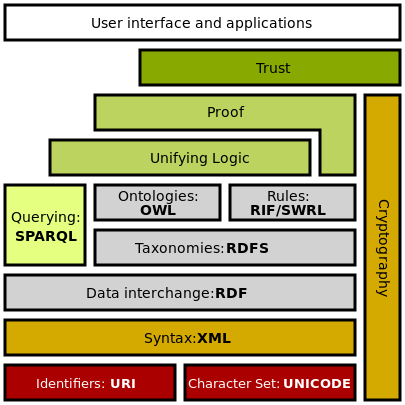
\includegraphics[width=0.75\linewidth]{img/Semantic_web_stack.png}
%     \caption{Semantic Web Stack}
%     \label{fig:bg:semantic-web-stack}
% \end{figure}

\subsection{RDF, RDFS, and OWL}

\subsubsection{Resource Description Framework (RDF)}
The representation of semantics starts with specification of facts or `knowledge' using RDF\footnote{\url{https://www.w3.org/TR/rdf11-concepts/}}, which provides representation of information as `triples' whose collective expression can be visualised as a graph.
RDF triples are serialised using syntax languages such as XML\footnote{\url{https://www.w3.org/TR/rdf-syntax-grammar/}}, or the more human-readable Turtle\footnote{\url{https://www.w3.org/TR/turtle/}}, or the web friendly JSON-LD\footnote{\url{https://www.w3.org/TR/json-ld/}}.
RDF triples utilise the same identifier system as world wide web and are specified using IRIs\footnote{\url{https://tools.ietf.org/html/rfc3987}} - a generalised form of URIs which itself are a generalised form of URLs\footnote{\url{https://www.w3.org/TR/uri-clarification/}}.
A database storing RDF is called a triple-store and enables creation of graphs of RDF data and provides an interface for querying it.

A RDF triple consists of a subject, an object, and a predicate - where predicate describes the relationship from subject to object. An example of RDF triple specified using the Turtle language to indicate chapter number of an entity is expressed as -\\ \-\hspace{5mm}\mintinline{turtle}{<http://example.com/ch2> foaf:name "Background"@en .}\\
The subject in this triple is the IRI \mintinline{turtle}{<http://example.com/ch2>} representing a resource, with the predicate \mintinline{turtle}{foaf:name} representing relationship of associating a name as indicated by the string in object field \mintinline{turtle}{"Background"@en} with \texttt{@en} specifying use of English language. 

The subject is written in shorthand notation indicating it starts with the same IRI as the data file it is described in. An IRI can become too long for readability and is usually written using shorthand prefixes.
The predicate is a \textit{property} provided by an external ontology called `Friend of a Friend' (FOAF\footnote{\url{http://xmlns.com/foaf/spec/}}), which is referenced by its prefix \texttt{foaf} as shorthand for its entire IRI.
The object is a string in this case, but could itself be another RDF triple or resource - in which case it would be specified as an IRI.

\subsubsection{RDF Schema (RDFS)}
RDFS provides concepts for expressing classes, properties, and data types in order to represent schemas using RDF. It also provides commonly required relationships such as specifying labels of resource, indicating related resource, or specifying domain and range of properties. The example in code below expands upon the triple described in RDF to express chapter as a class with its number as a property, and specifies human-readable labels for each resource.
\begin{minted}{turtle}
@prefix foaf: <http://xmlns.com/foaf/0.1/> .
@prefix : <http://example.com/> .
:Chapter rdf:type rdfs:Class ;
    rdfs:label "Chapter"@en .
:chnum a rdfs:Property ;
    rdfs:label "number"@en ;
    rdfs:range xsd:integer .
:Ch2 rdf:type :Chapter ;
    foaf:name "Background"@en ; 
    :chnum 2^^xsd:integer .
\end{minted}

\subsubsection{Web Ontology Language (OWL)}
While RDFS enables expression of hierarchies, more formal representations of knowledge modelling and logic require additional constructs. These are represented using OWL\footnote{\url{https://www.w3.org/TR/owl2-overview/}} as an ontology consisting of set of `individuals' (also called classes) and a set of `property assertions' which relate individuals to each other.
An ontology may also consist of set of axioms which place constraints on sets of individuals and types of relationships permitted between them. These axioms provide semantics which can be used to infer additional information using semantic reasoners based on information explicitly provided.
Knowledge expressed using OWL can be (and generally is) expressed using RDF, which makes it possible to encode and store ontologies in as RDF data.

\subsection{SPARQL Protocol and RDF Query Language (SPARQL)}
SPARQL\footnote{\url{https://www.w3.org/TR/sparql11-query/}} is a query language for retrieving data expressed using semantics provided by RDF.
SPARQL queries information following the RDF specification, and thus specifies queries to act on data expressed as `subject-predicate-object' triples.
SPARQL queries can also retrieve information from traditional (SQL) databases which store data in non-RDF form through mapping\footnote{\url{https://www.w3.org/2008/07/MappingRules/StemMapping}} which permits its semantics to be applied across a large variety of existing data stores.

A SPARQL endpoint is an interface for access and querying over stored data. Such endpoints can be exposed over the web to provide querying capabilities through the internet, with DBPedia\footnote{\url{http://dbpedia.org/sparql}} - a semantic web representation of Wikipedia - providing a well-known example.

\subsection{Shapes Constraint Language (SHACL)}
SHACL\footnote{\url{http://dbpedia.org/sparql}} is the W3C standard for expressing constraints that validate RDF data. The input over which SHACL constraints are validated is called the \textit{data graph}.
Constraints in SHACL are called `shapes' based on the notion of checking if data \textit{fits a shape}, with the set of constraints being validated called as \textit{shapes graph}.
SHACL constraints are themselves also expressed in RDF which makes it possible to serialise them as a data graph and perform querying over it.

The output of a validation process is a conformance report which uses a validation report vocabulary provided by SHACL and indicates \textit{failing validations} and status of validation of a whole. A \textit{conformance report} provides boolean indication of whether the any of given set of validations have failed or conversely whether all validations have passed.

\textit{SHACL core} refers to features defined within the SHACL standard specification. Extensions have been developed which provide additional features for expression and validation of constraints. \textit{SHACL-SPARQL} provides use of SPARQL queries to retrieve data failing a given constraint, and is mentioned within SHACL specification.
SHACL validations are performed using a `validator' - an implementation and interpretation of SHACL standard that provides at least the validation features described in SHACL-core.

Shape Expressions language (ShEx)\footnote{\url{https://www.w3.org/community/shex/}} is an alternative to SHACL that provides a similar conceptual language for expressing constraints and validating RDF data. The design of ShEx emphasises human readability inspired from Turtle, whereas SHACL follows the abstract RDF syntax. ShEx and SHACL were aimed to converge into a common standard, but this has not happened to date - and therefore both are maintained as separate technologies. Both SHACL and ShEx have seen significant adoption by the community.

\subsection{Standardised Ontologies}
\subsubsection{Provenance Ontology (PROV-O)}
PROV-O\footnote{\url{https://www.w3.org/TR/prov-o/}} is a standardised ontological representation of the PROV Data Model\footnote{\url{https://www.w3.org/TR/prov-dm/}} (PROV-DM) which is the W3C standard for representing provenance information using semantics provided by RDF and OWL.
PROV-O provides classes, properties, and restrictions to represent and interchange provenance information within different contexts.
It can be specialised to create new classes and properties to model provenance information for different applications and domains.

\subsubsection{Open Digital Rights Language (ODRL)}
ODRL\footnote{\url{https://www.w3.org/TR/odrl-model/}} is a policy expression language that provides an information model, vocabulary, and encoding mechanisms for representing statements about usage of content and services as policies. The ODRL Information Model describes underlying concepts, entities, and relationships that form the foundational basis for semantics of ODRL policies.
Policies are used to represent permitted and prohibited actions over one or more assets and can also contain obligations required to be met by stakeholders.
Policies can also specify constraints - such as temporal or spatial - and duties which are required to be carried out.
ODRL conformances is based on evaluating whether a given information representing an use-case or context satisfies all the expressions described in a given policy.